% Typeset with LaTeX format
% Using AMS extensions for mathematical formatting

%	The 'myarticle' class gives me a smaller title size
%	This class should appear as 'article'
%	in any submitted source file, so that others can
%	properly format it.  Please change if it is not correct.
%  	I use the 'leqno' option, for left-handed equation numbers.
\documentclass[leqno,11pt]{article}
%	To get all the formal devices, I usually use
%	all of 'amsmath', 'amssymb', and 'amsthm'.
%	There may also appear the packages
%	'setspace' (for double-spacing)
%	and 'mylogic' (for personal margins, headers, commands, etc.)
%	These should NOT appear in any submitted source file.
%	Please remove them if still here upon submission.
\usepackage{amsmath,amssymb,amsthm,amscd,amsxtra,latexsym}
\usepackage{enumerate}
\usepackage{graphicx}
\usepackage{hanging}
\usepackage[colorlinks=true,urlcolor=blue,linkcolor=black]{hyperref}
\usepackage{color}
\usepackage{tikz}
\usepackage{booktabs}


%---------------------------------------------
%       OPTIONAL:  PAGE SPACING HERE
%---------------------------------------------

%\usepackage{setspace}
%	The following line may be commented out
% 	If so, it can be deleted without affecting anything.
%	I use the command (with the 'setspace.sty' package)
%	for alternative formatting (also \doublespacing).
%	If this line is commented out, and 'setspace' is not in use,
%	the document formats as usual for its class.
%%\onehalfspacing

%---------------------------------------------
%       PAGE FORMAT (BORDERS/HEADERS)
%---------------------------------------------

%	Page format commands:
%	Override normal article margins,
%	making the margins smaller
\setlength{\textwidth}{6.5in}
\setlength{\textheight}{9in}
\setlength{\oddsidemargin}{0in}
\setlength{\evensidemargin}{0in}
\setlength{\topmargin}{-0.5in}

%---------------------------------------------
%       DEFINED COMMANDS
%---------------------------------------------

% A command for   'cardinality-of-XX' := |XX|
\newcommand{\card}[1]%
	{\ensuremath{\left| #1 \right|}}

% A command for 'set containing XX' := {XX}
\newcommand{\set}[1]%
	{\ensuremath{ \{ #1 \} }}

%	The 'such that' bar for set notation
\newcommand{\suth}{\ensuremath{ \,|\, }}

% A command for primes (')
\newcommand{\prm}%
	{\ensuremath{^{\prime}}}
		
% a command for double primes ('')
\newcommand{\pprm}%
	{\ensuremath{^{\prime \prime}}}

% A command for the Kleene star
\newcommand{\str}%
	{\ensuremath{^{\star}}}

% a command for the double star
\newcommand{\sstr}%
	{\ensuremath{^{\star\star}}}

% a command for question-numbers
\newcommand{\qn}[1]%
	{\noindent \textbf{[ #1 ]}\quad}
	
%---------------------------------------------
%       DOC STARTS HERE
%---------------------------------------------

\begin{document}

\begin{center}
{\large
\textbf{Computation Theory (CS 170), Section 01, Summer 2023} \\
\rule{0pt}{1em} \textbf{Assignment 01; due 11:59 PM Eastern, Wednesday, 7 June 2023}
}
\\
\hrulefill
\end{center}

\noindent 
Answer each of the following three questions to the best of your ability.  \textbf{Make sure that your
submission follows the formatting guidelines given at the end of this document.}

\vspace{4pt}\noindent 
You can find instructions for how to submit your work to Gradescope on the class website:
\begin{center}
	\href{https://canvas.tufts.edu/courses/48012/pages/how-to-submit-homework}
	{https://canvas.tufts.edu/courses/48012/pages/how-to-submit-homework}
\end{center}
 
\hrulefill 

\vspace{4pt}
\noindent 
In the following, we will assume (unless otherwise indicated) that we are using alphabet $\Sigma =
\set{\texttt{0},\, \texttt{1}}$.


\vspace{10pt}

\qn{1} (\emph{5 pts.}) Show that the following language is regular by constructing a DFA for it.
\[
	L_1 = \set{w \suth w \text{ contains the substring \texttt{101}}}
\]
\textbf{Note}: when you answer this question, provide both: (\emph{a}) the state diagram of the DFA, and
(\emph{b}) the full formal specification of the machine, as given by Definition $1.5$ (Sipser, 3rd ed., p.\
35).



(\emph{a})

\begin{center}

\begin{tikzpicture}[scale=0.2]
\tikzstyle{every node}+=[inner sep=0pt]
\draw [black] (16.1,-22.9) circle (3);
\draw (16.1,-22.9) node {$q0$};
\draw [black] (36.1,-34.7) circle (3);
\draw (36.1,-34.7) node {$q1$};
\draw [black] (45.8,-18.7) circle (3);
\draw (45.8,-18.7) node {$q2$};
\draw [black] (66.1,-18.8) circle (3);
\draw (66.1,-18.8) node {$q3$};
\draw [black] (66.1,-18.8) circle (2.4);
\draw [black] (7.5,-22.9) -- (13.1,-22.9);
\fill [black] (13.1,-22.9) -- (12.3,-22.4) -- (12.3,-23.4);
\draw [black] (18.68,-24.42) -- (33.52,-33.18);
\fill [black] (33.52,-33.18) -- (33.08,-32.34) -- (32.57,-33.2);
\draw (25.1,-29.3) node [below] {$1$};
\draw [black] (37.66,-32.13) -- (44.24,-21.27);
\fill [black] (44.24,-21.27) -- (43.4,-21.69) -- (44.26,-22.21);
\draw (41.59,-27.97) node [right] {$0$};
\draw [black] (48.8,-18.71) -- (63.1,-18.79);
\fill [black] (63.1,-18.79) -- (62.3,-18.28) -- (62.3,-19.28);
\draw (55.95,-19.25) node [below] {$1$};
\draw [black] (42.83,-19.12) -- (19.07,-22.48);
\fill [black] (19.07,-22.48) -- (19.93,-22.86) -- (19.79,-21.87);
\draw (30.61,-20.21) node [above] {$0$};
\draw [black] (39.073,-34.403) arc (123.44395:-164.55605:2.25);
\draw (43.18,-37.89) node [right] {$1$};
\fill [black] (38.14,-36.88) -- (38.17,-37.82) -- (39,-37.27);
\draw [black] (68.826,-20.024) arc (93.55967:-194.44033:2.25);
\draw (72.41,-24.5) node [below] {$0,\mbox{ }1$};
\fill [black] (66.79,-21.71) -- (66.34,-22.54) -- (67.34,-22.48);
\draw [black] (18.339,-24.879) arc (76.24902:-211.75098:2.25);
\draw (19.62,-29.66) node [below] {$0$};
\fill [black] (15.89,-25.88) -- (15.21,-26.54) -- (16.19,-26.78);
\end{tikzpicture}
\end{center}


(\emph{b})

$\Sigma = \set{\texttt{0},\, \texttt{1}}$

$Q = \set{\texttt{q0},\, \texttt{q1}, \texttt{q2}, \texttt{q3}}$

$q0 = \set{\texttt{q0}}$

$F = \set{\texttt{q3}}$


\begin{table}[h]
\begin{tabular}{@{}|l|ll@{}}
\toprule
$\delta$
\textbf{}   & \multicolumn{1}{l|}{\textbf{0}} & \multicolumn{1}{l|}{\textbf{1}} \\ \midrule
\textbf{q0} & q0                              & q1                              \\ \cmidrule(r){1-1}
\textbf{q1} & q2                              & q1                              \\ \cmidrule(r){1-1}
\textbf{q2} & q0                              & q3                              \\ \cmidrule(r){1-1}
\textbf{q3} & q3                              & q3                              \\ \bottomrule
\end{tabular}
\end{table}




\vspace{24pt}

\qn{2} (\emph{5 pts.}) The following regular language is formed of a combination of two simpler regular
languages.  Identify those two languages, and give state diagrams for DFA's that recognize each.  Then, combine
those DFA's into one for the more complex language, using the explicit procedure described in the Sipser text
(3rd ed., p.\ 46).
\[
	L_2 = \set{w \suth \card{w} \leq 2 \text{ and $w$ contains at least one \texttt{0}}} \\
\]
\textbf{Note}: when you design the two simpler machines, use different letters (like $q$ and $r$) for the states
of each, so it is more obvious how you have combined them into the final machine.  Also note that, unlike the
prior question, you \textbf{\emph{do not}} need a formal specification, only a diagram, for each machine.

\[
        A = \set{w \suth \card{w} \leq 2 } \\
\]
\[
	B = \set{w \suth \text{ $w$ contains at least one \texttt{0}}} \\
\]
\text{D(A):}
\begin{center}
\begin{tikzpicture}[scale=0.2]
\tikzstyle{every node}+=[inner sep=0pt]
\draw [black] (9.2,-23.2) circle (3);
\draw (9.2,-23.2) node {$r0$};
\draw [black] (9.2,-23.2) circle (2.4);
\draw [black] (25.5,-23.1) circle (3);
\draw (25.5,-23.1) node {$r1$};
\draw [black] (25.5,-23.1) circle (2.4);
\draw [black] (40.3,-23.1) circle (3);
\draw (40.3,-23.1) node {$r2$};
\draw [black] (40.3,-23.1) circle (2.4);
\draw [black] (56.6,-23.1) circle (3);
\draw (56.6,-23.1) node {$r3$};
\draw [black] (3.1,-23.2) -- (6.2,-23.2);
\fill [black] (6.2,-23.2) -- (5.4,-22.7) -- (5.4,-23.7);
\draw [black] (12.2,-23.18) -- (22.5,-23.12);
\fill [black] (22.5,-23.12) -- (21.7,-22.62) -- (21.7,-23.62);
\draw (17.35,-23.66) node [below] {$0,1$};
\draw [black] (28.5,-23.1) -- (37.3,-23.1);
\fill [black] (37.3,-23.1) -- (36.5,-22.6) -- (36.5,-23.6);
\draw (32.9,-23.6) node [below] {$0,1$};
\draw [black] (43.3,-23.1) -- (53.6,-23.1);
\fill [black] (53.6,-23.1) -- (52.8,-22.6) -- (52.8,-23.6);
\draw (48.45,-23.6) node [below] {$0,1$};
\draw [black] (58.492,-20.787) arc (168.44395:-119.55605:2.25);
\draw (63.47,-19.29) node [right] {$0,1$};
\fill [black] (59.59,-23.2) -- (60.27,-23.85) -- (60.47,-22.87);
\end{tikzpicture}
\end{center}


\text{D(B):}
\begin{center}
\begin{tikzpicture}[scale=0.2]
\tikzstyle{every node}+=[inner sep=0pt]
\draw [black] (9.3,-26.6) circle (3);
\draw (9.3,-26.6) node {$q0$};
\draw [black] (29.8,-26.6) circle (3);
\draw (29.8,-26.6) node {$q1$};
\draw [black] (29.8,-26.6) circle (2.4);
\draw [black] (2.9,-26.6) -- (6.3,-26.6);
\fill [black] (6.3,-26.6) -- (5.5,-26.1) -- (5.5,-27.1);
\draw [black] (12.3,-26.6) -- (26.8,-26.6);
\fill [black] (26.8,-26.6) -- (26,-26.1) -- (26,-27.1);
\draw (19.55,-27.1) node [below] {$0$};
\draw [black] (30.998,-23.862) arc (184.10091:-103.89909:2.25);
\draw (35.51,-20.81) node [right] {$0,1$};
\fill [black] (32.7,-25.89) -- (33.54,-26.33) -- (33.46,-25.33);
\draw [black] (8.729,-23.667) arc (218.74488:-69.25512:2.25);
\draw (11.85,-19.53) node [above] {$1$};
\fill [black] (11.28,-24.36) -- (12.22,-24.25) -- (11.59,-23.47);
\end{tikzpicture}
\end{center}

\text{D(A $\cap$ B):}
\begin{center}
\begin{tikzpicture}[scale=0.2]
\tikzstyle{every node}+=[inner sep=0pt]
\draw [black] (7.8,-25.7) circle (3);
\draw (7.8,-25.7) node {$q0$};
\draw [black] (7.8,-48.9) circle (3);
\draw (7.8,-48.9) node {$q1$};
\draw [black] (7.8,-48.9) circle (2.4);
\draw [black] (20.7,-14.9) circle (3);
\draw (20.7,-14.9) node {$r0$};
\draw [black] (20.7,-14.9) circle (2.4);
\draw [black] (37.5,-14.9) circle (3);
\draw (37.5,-14.9) node {$r1$};
\draw [black] (37.5,-14.9) circle (2.4);
\draw [black] (55.2,-14.9) circle (3);
\draw (55.2,-14.9) node {$r2$};
\draw [black] (55.2,-14.9) circle (2.4);
\draw [black] (69.2,-14.9) circle (3);
\draw (69.2,-14.9) node {$r3$};
\draw [black] (20.7,-25.7) circle (3);
\draw (20.7,-25.7) node {$r0q0$};
\draw [black] (19.9,-48.9) circle (3);
\draw (19.9,-48.9) node {$r0q1$};
\draw [black] (19.9,-48.9) circle (2.4);
\draw [black] (36.8,-25.7) circle (3);
\draw (36.8,-25.7) node {$r1q0$};
\draw [black] (55.2,-25.7) circle (3);
\draw (55.2,-25.7) node {$r2q0$};
\draw [black] (70.8,-25.7) circle (3);
\draw (70.8,-25.7) node {$r3q0$};
\draw [black] (36,-48.9) circle (3);
\draw (36,-48.9) node {$r1q1$};
\draw [black] (36,-48.9) circle (2.4);
\draw [black] (53.4,-48.9) circle (3);
\draw (53.4,-48.9) node {$r2q1$};
\draw [black] (53.4,-48.9) circle (2.4);
\draw [black] (69.8,-48.9) circle (3);
\draw (69.8,-48.9) node {$r3q1$};
\draw [black] (1.4,-25.7) -- (4.8,-25.7);
\fill [black] (4.8,-25.7) -- (4,-25.2) -- (4,-26.2);
\draw [black] (7.8,-28.7) -- (7.8,-45.9);
\fill [black] (7.8,-45.9) -- (8.3,-45.1) -- (7.3,-45.1);
\draw (7.3,-37.3) node [left] {$0$};
\draw [black] (5.162,-47.496) arc (269.70529:-18.29471:2.25);
\draw (2.11,-42.92) node [above] {$0,1$};
\fill [black] (7.31,-45.95) -- (7.81,-45.15) -- (6.81,-45.15);
\draw [black] (4.983,-24.703) arc (278.23895:-9.76105:2.25);
\draw (2.07,-20.38) node [above] {$1$};
\fill [black] (6.88,-22.86) -- (7.26,-21.99) -- (6.27,-22.14);
\draw [black] (13.2,-14.9) -- (17.7,-14.9);
\fill [black] (17.7,-14.9) -- (16.9,-14.4) -- (16.9,-15.4);
\draw [black] (23.7,-14.9) -- (34.5,-14.9);
\fill [black] (34.5,-14.9) -- (33.7,-14.4) -- (33.7,-15.4);
\draw (29.1,-14.4) node [above] {$0,1$};
\draw [black] (40.5,-14.9) -- (52.2,-14.9);
\fill [black] (52.2,-14.9) -- (51.4,-14.4) -- (51.4,-15.4);
\draw (46.35,-14.4) node [above] {$0,1$};
\draw [black] (58.2,-14.9) -- (66.2,-14.9);
\fill [black] (66.2,-14.9) -- (65.4,-14.4) -- (65.4,-15.4);
\draw (62.2,-14.4) node [above] {$0,1$};
\draw [black] (69.016,-11.917) arc (211.2532:-76.7468:2.25);
\draw (73.5,-8.15) node [above] {$0,1$};
\fill [black] (71.46,-12.94) -- (72.4,-12.95) -- (71.88,-12.1);
\draw [black] (14.8,-25.7) -- (17.7,-25.7);
\fill [black] (17.7,-25.7) -- (16.9,-25.2) -- (16.9,-26.2);
\draw [black] (23.7,-25.7) -- (33.8,-25.7);
\fill [black] (33.8,-25.7) -- (33,-25.2) -- (33,-26.2);
\draw (28.75,-26.2) node [below] {$1$};
\draw [black] (22.35,-28.2) -- (34.35,-46.4);
\fill [black] (34.35,-46.4) -- (34.33,-45.45) -- (33.49,-46);
\draw (27.74,-38.63) node [left] {$0$};
\draw [black] (22.9,-48.9) -- (33,-48.9);
\fill [black] (33,-48.9) -- (32.2,-48.4) -- (32.2,-49.4);
\draw (27.95,-49.4) node [below] {$0,1$};
\draw [black] (39,-48.9) -- (50.4,-48.9);
\fill [black] (50.4,-48.9) -- (49.6,-48.4) -- (49.6,-49.4);
\draw (44.7,-49.4) node [below] {$0,1$};
\draw [black] (56.4,-48.9) -- (66.8,-48.9);
\fill [black] (66.8,-48.9) -- (66,-48.4) -- (66,-49.4);
\draw (61.6,-49.4) node [below] {$0,1$};
\draw [black] (71.887,-46.761) arc (163.44003:-124.55997:2.25);
\draw (76.93,-45.9) node [right] {$0,1$};
\fill [black] (72.77,-49.26) -- (73.39,-49.96) -- (73.68,-49);
\draw [black] (39.8,-25.7) -- (52.2,-25.7);
\fill [black] (52.2,-25.7) -- (51.4,-25.2) -- (51.4,-26.2);
\draw (46,-26.2) node [below] {$1$};
\draw [black] (58.2,-25.7) -- (67.8,-25.7);
\fill [black] (67.8,-25.7) -- (67,-25.2) -- (67,-26.2);
\draw (63,-26.2) node [below] {$1$};
\draw [black] (38.55,-28.14) -- (51.65,-46.46);
\fill [black] (51.65,-46.46) -- (51.6,-45.52) -- (50.78,-46.1);
\draw (44.51,-38.67) node [left] {$0$};
\draw [black] (56.8,-28.24) -- (68.2,-46.36);
\fill [black] (68.2,-46.36) -- (68.2,-45.42) -- (67.35,-45.95);
\draw (61.87,-38.6) node [left] {$0$};
\draw [black] (71.761,-22.871) arc (188.96706:-99.03294:2.25);
\draw (76.1,-19.45) node [right] {$0,\mbox{ }1$};
\fill [black] (73.63,-24.74) -- (74.5,-25.11) -- (74.34,-24.12);
\end{tikzpicture}
\end{center}

\vspace{24pt}

\qn{3} (\emph{5 pts.}) Consider the following NFA, on the 3-character alphabet $\Sigma = \set{\texttt{0},
\texttt{1}, \texttt{2}}$:
\begin{center}
\begin{tikzpicture}[scale=0.2]
\tikzstyle{every node}+=[inner sep=0pt]
\draw [black] (7.7,-14.6) circle (3);
\draw (7.7,-14.6) node {$a$};
\draw [black] (22.3,-14.6) circle (3);
\draw (22.3,-14.6) node {$b$};
\draw [black] (39.6,-14.6) circle (3);
\draw (39.6,-14.6) node {$c$};
\draw [black] (39.6,-14.6) circle (2.4);
\draw [black] (30.9,-26.5) circle (3);
\draw (30.9,-26.5) node {$d$};
\draw [black] (2.3,-14.6) -- (4.7,-14.6);
\fill [black] (4.7,-14.6) -- (3.9,-14.1) -- (3.9,-15.1);
\draw [black] (10.7,-14.6) -- (19.3,-14.6);
\fill [black] (19.3,-14.6) -- (18.5,-14.1) -- (18.5,-15.1);
\draw (15,-14.1) node [above] {$\varepsilon$};
\draw [black] (32.67,-24.08) -- (37.83,-17.02);
\fill [black] (37.83,-17.02) -- (36.95,-17.37) -- (37.76,-17.96);
\draw (34.67,-19.16) node [left] {$\varepsilon$};
\draw [black] (24.06,-17.03) -- (29.14,-24.07);
\fill [black] (29.14,-24.07) -- (29.08,-23.13) -- (28.27,-23.71);
\draw (26.01,-21.93) node [left] {\texttt{1}};
\draw [black] (42.28,-13.277) arc (144:-144:2.25);
\draw (46.85,-14.6) node [right] {\texttt{2}};
\fill [black] (42.28,-15.92) -- (42.63,-16.8) -- (43.22,-15.99);
\draw [black] (25.3,-14.6) -- (36.6,-14.6);
\fill [black] (36.6,-14.6) -- (35.8,-14.1) -- (35.8,-15.1);
\draw (30.95,-14.1) node [above] {\texttt{2}};
\draw [black] (6.377,-11.92) arc (234:-54:2.25);
\draw (7.7,-7.35) node [above] {\texttt{0}};
\fill [black] (9.02,-11.92) -- (9.9,-11.57) -- (9.09,-10.98);
\draw [black] (33.58,-25.177) arc (144:-144:2.25);
\draw (38.15,-26.5) node [right] {\texttt{1}};
\fill [black] (33.58,-27.82) -- (33.93,-28.7) -- (34.52,-27.89);
\end{tikzpicture}
\end{center}
Give a precise definition of the language of this machine.  Then, use the procedure of Theorem $1.39$, (Sipser,
3rd ed., p. 55f) to convert it to a corresponding DFA.  Give the final DFA diagram.

\vspace{4pt} \noindent
\textbf{Note}: here, the DFA can get quite large, and involves a number of unreachable states.  For full points,
all such states should be \textbf{\emph{excluded}} from the diagram, to keep it simpler.

\[
	L = \set{w \suth {w} \text{ ends with 2 and the only 0's are leading}} \\
\]


\begin{center}
\begin{tikzpicture}[scale=0.2]
\tikzstyle{every node}+=[inner sep=0pt]
\draw [black] (24.5,-45.7) circle (3);
\draw (24.5,-45.7) node {$ab$};
\draw [black] (25.5,-5.8) circle (3);
\draw (25.5,-5.8) node {$dc$};
\draw [black] (24.5,-25.2) circle (3);
\draw (24.5,-25.2) node {$c$};
\draw [black] (24.5,-25.2) circle (2.4);
\draw [black] (53.1,-25.2) circle (3);
\draw (53.1,-25.2) node {$\theta$};
\draw [black] (15.7,-45.7) -- (21.5,-45.7);
\fill [black] (21.5,-45.7) -- (20.7,-45.2) -- (20.7,-46.2);
\draw [black] (21.753,-44.5) arc (-117.69687:-245.17449:20.992);
\fill [black] (22.7,-6.86) -- (21.76,-6.74) -- (22.18,-7.65);
\draw (9.99,-25.38) node [left] {$1$};
\draw [black] (27.95,-7.53) -- (50.65,-23.47);
\fill [black] (50.65,-23.47) -- (50.28,-22.61) -- (49.7,-23.42);
\draw (38.3,-16) node [below] {$0$};
\draw [black] (25.35,-8.8) -- (24.65,-22.2);
\fill [black] (24.65,-22.2) -- (25.19,-21.43) -- (24.2,-21.38);
\draw (24.42,-15.48) node [left] {$2$};
\draw [black] (21.59,-24.522) arc (284.61535:-3.38465:2.25);
\draw (18.73,-19.49) node [left] {$2$};
\fill [black] (23.27,-22.48) -- (23.55,-21.58) -- (22.58,-21.83);
\draw [black] (24.5,-42.7) -- (24.5,-28.2);
\fill [black] (24.5,-28.2) -- (24,-29) -- (25,-29);
\draw (25,-35.45) node [right] {$2$};
\draw [black] (27.5,-25.2) -- (50.1,-25.2);
\fill [black] (50.1,-25.2) -- (49.3,-24.7) -- (49.3,-25.7);
\draw (38.8,-25.7) node [below] {$0,\mbox{ }1$};
\draw [black] (26.909,-43.932) arc (154.00798:-133.99202:2.25);
\draw (31.87,-44.27) node [right] {$0$};
\fill [black] (27.37,-46.54) -- (27.87,-47.34) -- (28.31,-46.44);
\draw [black] (27.497,-3.577) arc (165.80141:-122.19859:2.25);
\draw (32.51,-2.41) node [right] {$1$};
\fill [black] (28.48,-6.03) -- (29.13,-6.71) -- (29.38,-5.74);
\end{tikzpicture}
\end{center}



\hrulefill 

\begin{center}
	\emph{Formatting instructions appear on the following page.}
\end{center}
 
 \pagebreak 

\noindent 
\textbf{Format requirements}: work should correspond to the following guidelines:
\begin{itemize}  

	\item Work must be in type-written format, with any diagrams rendered using software to produce
		professional-looking results.  No hand-written or hand-drawn work will be graded.
		
	\item Work must be submitted in PDF format to Gradescope.

\end{itemize}

\vspace{4pt}\noindent 
You can find links to information about using LaTeX to produce type-written mathematical work,\footnote{LaTeX
was used to produce this document.}  on the class website:
\begin{center}
	\href{https://canvas.tufts.edu/courses/48012/pages/latex-document-preparation}
	{https://canvas.tufts.edu/courses/48012/pages/latex-document-preparation}
\end{center}
While you can use any drawing/layout program to produce images, there is a handy web-based tool for drawing
finite-state diagrams for DFA/NFA that produces nice results (the image in this assignment was generated using
that tool, exporting the code for the image to LaTeX for inclusion):
\begin{center}
	\href{http://madebyevan.com/fsm/}{http://madebyevan.com/fsm/}
\end{center}
 
\end{document}
 
